\documentclass[../PhD.tex]{subfiles}

\begin{document}

%%%%%%%%%%%%%%%%%%%%%%%%%%%%%%%%%%%%%%%%%%%%%%%%%%%%%%
%%%%%%%%%%%%%%%%%%%%%%%%%%%%%%%%%%%%%%%%%%%%%%%%%%%%%%

\chapter{Introduction}
\label{ch: intro}

As experimental research into quantum information, condensed matter, and nuclear physics continues to reach new levels of precision, progress in developing theoretical predictions in these fields is hindered by a fundamental flaw: in strong coupling regimes, the perturbative methods that underpin theories such as Quantum Electrodynamics become invalid. This is because such systems are highly nonlinear. While some progress is possible by employing numerical schemes such as lattice approximations, analytical results are beyond our current mathematical understanding. It was not until a result derived from string theory -- and hinted at by studies of emergent gravity in gauge theories -- was developed that  strongly coupled phases of matter could be investigated analytically. By considering different coupling limits of a single string theory, a holographic description between strongly-coupled gauge theories and weakly-coupled gravitational theories in one higher dimension was established. Since its inception, this duality has been further developed into a dictionary that relates the fields in the gravitational theory to operators in the gauge theory. Thus, the Anti-de Sitter/Conformal Field Theory (AdS/CFT) correspondence allows strongly-coupled quantum processes to be reliably examined via geometric quantities in the dual theory. This duality has become a standard tool for theoretical physicists studying all kinds of dynamic processes in quantum theories, in particular the analysis of out-of-equilibrium dynamics at strong coupling. What the AdS/CFT correspondence is, and what it can tell us about dynamical processes in quantum field theories, will be the subject of this review.

This document is organized as follows. In \S~\!\ref{sec: ads/cft} we wish to motivate the existence of a duality between a conformal field theory in $d$-dimensions and a negative-curvature gravitational theory in ($d + 1$)-dimensions. After examining a particular instance of this duality, we will discuss a few of the entries in the AdS/CFT dictionary that will prove useful later on. In \S~\!\ref{sec: bh in ads}, we see how black holes fit in to the AdS/CFT correspondence and examine how they can be used to describe a thermal state of a gauge theory. Finally, Section~\ref{sec: grav collapse} focuses on the modelling of dynamic processes in the gauge theory via the collapse of scalar fields in AdS. We discuss the holographic description of quantum quenches and revivals, describing current research into both analytic and numerical solutions in AdS.

%%%%%%%%%%%%%%%%%%%%%%%%%%%%%%%%%%%%%%%%%%%%%%%%%%%%%%%
%%%%%%%%%%%%%%%%%%%%%%%%%%%%%%%%%%%%%%%%%%%%%%%%%%%%%%%

\section{The AdS/CFT Correspondence}
\label{sec: ads/cft}

The AdS/CFT correspondence was first established by \cite{hep-th/9711200}, who studied two limits of type IIb string theory and found that the low-energy states in either limit described either a supergravity theory with a negative cosmological constant, or a superconformal quantum field theory living on the boundary of the gravity theory. Although this correspondence was originally conjectured from the point of view of string theory, more modern reviews of the duality rely less on the specifics of the string theory and instead develop a gravitational theory from the strong coupling limit of a gauge theory \cite{gr-qc/0602037}. We will use this paradigm to heuristically motivate the duality, as well as introduce relevant relationships between quantities in either theory.  

%%%%%%%%%%%%%%%%%%%%%%%%%%%%%%%%%%%%%%%%%%%%%%%%%%%%%%%

\subsection{Extra Dimensions In Gauge Theories}
\label{ssec: extra dims in gauge theories}

Although \cite{hep-th/9711200} was the first to establish explicitly a correspondence between a gravitational theory in $(d+1)$-dimensional AdS and a conformal field theory in $d$-dimensions, the concept of a holographic relationship between a gauge theory and a gravitational theory in one higher dimension was established earlier by \cite{gr-qc/9310026} and \cite{hep-th/9409089} from the point of view of the field theory. 

For most gauge theories, there is a running of the coupling that dictates the evolution of the couplings with energy. Therefore, the physics of the theory is local with respect to an extra dimension, the energy. However, since many gauge theories suffer UV divergences at large energies, the size of the extra dimension may be limited. In contrast, supersymmetric theories have vanishing beta functions; therefore, there is no running of the coupling. In this case, the energy scale is arbitrary and the extra dimension of the theory has no bound.

The vanishing of the beta function also indicates that the conformal invariance of the theory is unbroken; conformal invariance requires (among other things) that the theory remain invariant under rigid scale transformations $x^\mu \to \ell x^\mu$. Interpreting the energy scale as an extra dimension, $r$, we require it to transform as $r \to r/ \ell$. The most generic metric that also obeys Poincar\'e plus scale symmetries is
\begin{align}
\label{Poincare ads}
ds^2 = \frac{\ell^2}{z^2} \left( \eta_{\mu \nu}dx^\mu dx^\nu +dz^2 \right) \, ,
\end{align}
where $z = \ell^2 / r$. This is precisely the metric for AdS$_5$ with characteristic length $\ell$. 

While this argument is for a specific gauge theory, the gauge/gravity correspondence is in fact a much deeper and wider relationship. The derivation of the duality is thoroughly covered from the full string theory perspective in, among others, \cite{hep-th/9711200, gr-qc/0602037, 1501.00007, hep-th/9902131, hep-th/9905111}. For now, let us establish the duality that will be most applicable to us: the duality between type IIb supergravity on conformal AdS$_5 \times$ S$^5$ and $\mc N = 4$ supersymmetric Yang-Mills theory in $(3+1)$-dimensions.

%%%%%%%%%%%%%%%%%%%%%%%%%%%%%%%%%%%%%%%%%%%%%%%%%%%%%%%

\subsection{The AdS$_5 \times$S$^5$ Duality}
\label{ssec: AdS5xS5}

Consider a stack of $N$ coincident D3-branes in type IIb string theory (ten Minkowski dimensions), each of which couple to gravity with strength $g_s$. At weak coupling, $g_s N \ll 1$, there are closed string states as well as open strings that end on the branes and have an $SU(N)$ super-Yang-Mills effective action \cite{Zwiebach:2004tj}. At strong coupling, however, the branes curve the background and source an extremal black-brane geometry \cite{Horowitz:1991cd}, whose metric is
\begin{align}
\label{bb geom}
ds^2 = f(r)^{-1/2} \eta_{\mu \nu} dx^\mu dx^\nu + f(r)^{1/2} \left(  dr^2 + r^2 d\Omega_5^2 \right)  \quad  \text{with} \quad f(r) = 1 + \frac{4 \pi g_s N \ell_s^4}{r^4} \, ,
\end{align}
where the $x^\mu$ span the worldvolume of the D3-branes and $d\Omega_5^2$ is the metric of the unit 5-sphere.

Now we take the low-energy limit of the theories at either coupling limit. At weak coupling, the open strings decouple from the closed strings, resulting in an $SU(N)$ super-Yang-Mills gauge theory on the brane worldvolume. In the $g_s N \gg 1$ case, the low-energy limit corresponds to the near-horizon limit, $r \to 0$. In this limit, the 10D metric factors into the product AdS$_5 \times$S$^5$ ({\it cf.} the near-horizon limit of an extremal Reissner-Nordstr\o m black hole in $d=4$ \cite{Horowitz:1991cd}). To see this, we define\footnote{ This definition is actually derivable, and is motivated above equation \eqref{params}.} $\ell \equiv (4\pi g_s N)^{1/4} \ell_s$, so that $f^{1/2}(r) \to \ell^2 / r^2$ in the near-horizon limit and \eqref{bb geom} becomes
\begin{align}
\label{param rels}
ds^2 = \frac{r^2}{\ell^2} \eta_{\mu \nu} dx^\mu dx^\nu + \frac{\ell^2}{r^2}dr^2 + \ell^2 d\Omega_5^2 \, .
\end{align}
Note that the branes are now located at the bottom of the infinite throat. Any states near the horizon will be redshifted to low energies and any states in the asymptotic region will decouple from states near the black branes; all that remains are closed string states, {\it i.e.} supergravity, on an asymptotically AdS$_5$ background. This motivates the duality we will examine in detail: the one between scalar fields in \ads and a supersymmetric $SU(N)$ Yang-Mills gauge theory on the boundary of AdS$_5$.

Given that we now know what string theory we are working with, we can more directly relate the dimensionless parameters of the string theory ({\it i.e.}, the string coupling $g_s$ and AdS scale in string units, $\ell / \ell_s$) to the dimensionless parameters of the CFT ({\it i.e.}, the Yang-Mills coupling $g_{YM}$ and colour number $N$). By examining the D3-brane Lagrangian, we are able to relate $g_{YM}$ and $g_s$ through $4\pi g_s = g_{YM}^2$. Furthermore, since each D3-brane sources a 5-form field strength, quantization of the flux through the five-sphere S$^5$ leads to an expression for the radius of curvature of AdS. Altogether,
\begin{align}
\label{params}
4\pi g_s = g_{YM}^2 \sim \frac{\lambda}{N} \quad \text{and} \quad \frac{\ell}{\ell_s} = \left( 4\pi g_s N \right)^{1/4} \sim \lambda^{1/4} \, ,
\end{align}
where $\lambda$ is the 't Hooft coupling $\lambda \equiv g_s N = g_{YM}^2 N$, and $\ell_s$ is the string length. To remove stringy corrections to the geometry, $\ell / \ell_s \gg 1$ so that the AdS length is much larger than the string length. Furthermore, string interactions are suppressed when $g_s \ll 1$. Thus, the bulk theory approaches  classical Einstein-Hilbert gravity when $N \gg \lambda \gg 1$.

%%%%%%%%%%%%%%%%%%%%%%%%%%%%%%%%%%%%%%%%%%%%%%%%%%%%%%%

\subsection{The Gauge/Gravity Dictionary}
\label{ssec: dictionary}

With the existence of the duality now motivated, we turn to what can be directly related through the correspondence. In particular, we wish to ask: \emph{what physical quantities in either theory can be related through the AdS/CFT correspondence?} In fact, many such relations arose from efforts to find counterexamples to the correspondence in the hopes of disproving it. Instead, each attempt confirmed the AdS/CFT correspondence and became an entry in the so-called dictionary. Here we will provide a few such examples.

\subsubsection*{Symmetries}
Consider the symmetries present in the \ads bulk theory. A $(p+2)$-dimensional Anti-de Sitter space can be presented by the hyperboloid $X_0^2 + X^2_{p+2} - \sum^{p+1}_{i=1} X_i^2 = \ell^2$ in a $(p+3)$-dimensional space with the metric
\begin{align}
\label{ads hyperboloid}
ds^2 = -dX_0^2 - dX_{p+2}^2 + \sum^{p+1}_{i = 1} dX^2_i \, .
\end{align}
This space has a $SO(2,p+1)$ isometry group \cite{hep-th/9905111}. Thus, the \ads theory has $SO(2,4)\times SO(6)$ symmetry. On the other hand, the gauge theory has an $SO(2,4)$ isometry from its conformal invariance (Poincar\'e plus scale and special conformal transformations) as well as $SU(4) \simeq SO(6)$ R-symmetry that relates the six scalar fields and four fermions of the theory \cite{1501.00007}. Therefore, the spatial isometries of the bulk space are interpreted as global symmetries of the boundary theory. Additionally, the supersymmetries inherent in the original theory type IIb superstring theory remain unbroken by the strong/weak coupling limits.
	
\subsubsection*{Observables}
\label{ssub: lengths}

Besides matching symmetry groups and relating dimensionless parameters, the AdS/CFT correspondence is able to produce more physically relevant relationships involving observables in either theory. One such concrete example comes from relating the asymptotic behaviour of bulk fields to the expectation values of operators in the boundary theory: a bulk field with leading-order value $\phi^{(0)}$ as $z \to 0$ acts as a source for an operator $\mc O$ on the boundary. Furthermore, by examining the next-to-leading order contribution to the bulk field, $\phi^{(1)}$, it can be shown that the expectation value of the operator is given by $\langle \mc O \rangle \propto \phi^{(1)}$ \cite{hep-th/9905104}. In \S~\!\ref{ssec: scalar fields}, we use the gauge/gravity duality to calculate the mass dimension of the boundary operator $\mc O$.

Another such example is the quark anti-quark potential in the boundary theory. In the gauge theory, this can be calculated via the Wilson loop $W(\mathcal C)$, where $\mathcal C$ is the closed loop connecting the quark worldlines. The bulk interpretation of the Wilson loop is the extremized proper area of a string worldsheet anchored on $\mathcal C$ and extending into $z > 0$ \cite{hep-th/9803002}. 


\subsubsection*{Entanglement Entropy}
\label{ssub: EE}
A significant utilization of the gauge/gravity duality comes from its unique ability to relate quantum characteristics of the gauge theory to geometric ones in the bulk. Among the most quantum of all characteristics is the spatial distribution of quantum correlations within a system, given by the entanglement entropy. For a given subsystem $\mc M$ of a local field theory with reduced density matrix $\rho_{\mc M}$, the entanglement entropy is given by the Von Neumann entropy $S_{\mc M} = - \text{Tr} \rho_{\mc M} \ln \rho_{\mc M}$. In practice, $\mc M$ is a spatial region that is bounded by the entangling surface $\p \mc M$.

In the strong coupling limit, calculating the entanglement entropy can be prohibitively difficult. However, using the AdS/CFT correspondence, and an analogous process to the Wilson loop calculation discussed in \S~\!\ref{ssub: lengths}, it has been shown that $S_{\mc M}$ is given by a quarter of the area of the minimal surface at constant time in the bulk that is anchored on $\p \mc M$ \cite{hep-th/0603001}. Further properties of the entanglement entropy were subsequently shown to also have dual geometric descriptions in the bulk \cite{1304.4926}. In \S~\!\ref{sub: quenches}, we will see how entanglement entropy can also be calculated out of equilibrium, yielding the time-dependent entanglement behaviour of the strongly-coupled quantum theory.

\subsubsection*{Partition Functions}
\label{ssec: partitions}

Since the underpinning of the AdS/CFT correspondence is taking different limits of the same theory, it is natural that the partition functions of either limit must still agree. We have already seen in \S~\!\ref{ssec: AdS5xS5} that the weak coupling limit of the type IIb string theory is supergravity (SUGRA) in the bulk, while the strong coupling limit gives a supersymmetric (SUSY) Yang-Mills gauge theory on the boundary. The gauge/gravity duality allows us to relate the two limits of the partition function:
\begin{align}
\label{partition functions}
e^{-S_{SUGRA}} \approx Z_{string} \simeq Z_{gauge} = e^{-W_{SUSY}} \, ,
\end{align}
where $W$ is the generating functional for connected Green's functions in the gauge theory.

Consider a bulk field $\phi(\vec x,z)$ with boundary value $\phi(\vec x, z=0) = \phi_0 (\vec x)$. We then solve the bulk equations of motion away from the boundary ({\it i.e.}, $z > \epsilon$) and subject to the Dirichlet condition $\phi(\vec x, z=\epsilon) \to \phi_0(\vec x)$ as $\epsilon \to 0$. By definition, $S_{SUGRA}$ is extremized by this solution and so \eqref{partition functions} becomes \cite{hep-th/9802109, hep-th/9802150}
\begin{align}
\label{ads/cft duality}
\lim_{\epsilon \to 0} \big( S_{SUGRA} \left[ \phi(\vec x, z) \right] \big) \Big|_{\phi (\vec x, \epsilon) \to \phi_0(\vec x)} \simeq \left\langle \int d^dx \, \phi_0(\vec x) \mc O(\vec x) \right\rangle_{CFT} \, .
\end{align}
Let us now see what results can be derived from this duality for a scalar field in AdS$_{d+1}$.

%%%%%%%%%%%%%%%%%%%%%%%%%%%%%%%%%%%%%%%%%%%%%%%%%%%%%%%

\subsection{Solutions For Scalar Fields in AdS$_{d+1}$}
\label{ssec: scalar fields}

To determine the solution for a massive scalar field $\phi(\vec x, z)$ in AdS$_{d+1}$ space, we begin with the bulk action for the free field
\begin{align}
\label{free field act}
S[\phi] = -\frac{G^{(d+1)}}{2} \int d^{d+1} x \, \sqrt{g} \left( g^{AB} \p_A \phi \p_B \phi + m^2 \phi^2 + \ldots \right) \, ,
\end{align}
where $G^{(d+1)}$ is the ($d+1$)-dimensional Newton's constant. Note that any higher-order terms in $\phi$ have been suppressed. The bulk metric written in Poinar\'e patch coordinates is as presented in \S~\!\ref{ssec: extra dims in gauge theories}. When integrating \eqref{free field act} by parts we must be careful to retain any surface terms since they will not go to zero like the flat-space case. With this is mind, we find that
\begin{align}
\label{action int by parts}
S[\phi] = -\frac{G^{(d+1)}}{2} \int d^{d+1}x \, \sqrt{g}\, \phi \left( - \Box + m^2 \right) \phi - \frac{G^{(d+1)}}{2}\int_{\p AdS} d^d x \sqrt{\gamma} \, g^{zB} \phi \, \p_B \phi \, ,
\end{align}
with $\Box \phi = g^{-1/2} \p_A (\sqrt{g} \, g^{AB} \p_B) \phi$ and $\gamma$ equal to the induced metric on the boundary. Taking $\phi(\vec x, z)$ to be of the form $\phi(\vec x, z) = \exp( i k_\mu x^\mu) f_k (z)$, the wave equation becomes
\begin{align}
\label{bessel}
0 &= \frac{1}{\ell^2} \left( z^2 k^2 - z^{d} \p_z (z^{-d} \p_z ) + m^2 \ell^2 \right) f_k(z) \, .
\end{align}
The solutions to \eqref{bessel} are Bessel functions, but for now it suffices to examine only their limiting behaviour. Near the boundary the solutions scale like a power law in $z$, and substituting $f_k(z) \propto z^{\Delta}$ into the equation above gives
\begin{align}
0 = \left(k^2 z^2 - \Delta(\Delta - d) + m^2 \ell^2 \right) z^\Delta \, .
\end{align}
Or, in the limit $z \to 0$,
\begin{align}
\label{Delta roots}
m^2 \ell^2 = \Delta (\Delta - d) \qquad \Rightarrow \qquad \Delta^{\pm} = \frac{d}{2} \pm \sqrt{\frac{d^2}{4} + m^2\ell^2} \, .
\end{align}
{\it N.B.} requiring that the energies of scalar fields in the bulk be real means that the factor inside the square root of \eqref{Delta roots} is either positive or zero. The mass-squared must then be $m^2 \ell^2 \geq - d^2 /4$, which is known as the Breitenlohner-Freedman bound \cite{Breitenlohner:1982bm}. Of the two values permitted by \eqref{Delta roots}, $\Delta^+$ remains positive for all dimensions and therefore the solution $z^{\Delta^+}$ scales appropriately as $z \to 0$. However, the $z^{\Delta^-}$ solution may cause the scalar field to diverge at the boundary. To avoid this, we modify the boundary condition for $\phi(\vec x, z=0)$ to be
\begin{align}
\label{scalar bc}
\phi(\vec x, z=0) = \lim_{\epsilon \to 0} \phi(\vec x, z=\epsilon) = \lim_{\epsilon \to 0} \epsilon^{\Delta^-} \phi_0 (\vec x) \, ,
\end{align}
where $\phi_0 (\vec x)$ is the renormalizable field on the boundary. 

We can use \eqref{scalar bc} to motivate the scaling dimension of $\mc O (\vec x)$, which tells us how relevant that operator remains with renormalization group flow. First, note that the induced metric in \eqref{action int by parts} is
\begin{align}
ds^2 \Big|_{z=\epsilon} = \frac{\ell^2}{\epsilon^2} \eta_{\mu \nu} dx^\mu dx^\nu = \gamma_{\mu \nu} dx^\mu dx^\nu \, ,
\end{align}
and that the coupling between the field and the operator given in \eqref{ads/cft duality} is more correctly written in terms of a limit of a bulk interaction. Using the scaling behaviour of $\phi$ near the boundary, we see that
\begin{align}
\lim_{\epsilon \to 0} \int_{z=\epsilon} d^{d}x \sqrt{\gamma} \, \phi(\vec x, z = \epsilon) \mc O(\vec x, \epsilon) = \lim_{\epsilon \to 0} \int_{\p AdS} d^d x \left(\frac{\ell}{\epsilon}\right)^d \left( \epsilon^{\Delta^-} \phi_0 (\vec x) \right) \mc O (\vec x, \epsilon) \, .
\end{align}
Since the action must be finite as $\epsilon \to 0$, we have that $ \mc O(\vec x, \epsilon) \sim \epsilon^{d} \epsilon^{-\Delta^-} \mc O_0 (\vec x) = \epsilon^{d - \Delta^-} \mc O_0 (\vec x) = \epsilon^{\Delta^+} \mc O_0 (\vec x)$, where $\mc O_0(\vec x)$ is the normalizable operator in the CFT. The relevance of the operator will be determined by the value of $\Delta^+$.


%%%%%%%%%%%%%%%%%%%%%%%%%%%%%%%%%%%%%%%%%%%%%%%%%%%%%%%
%%%%%%%%%%%%%%%%%%%%%%%%%%%%%%%%%%%%%%%%%%%%%%%%%%%%%%%
	
\section{Black Holes and the AdS/CFT Correspondence}
\label{sec: bh in ads}

Our primary application of the AdS/CFT correspondence will be to examine in detail various processes in the bulk given that we have a dictionary to translate the solutions to the boundary gauge theory. In particular, we wish to consider thermal states of the CFT which have a dual description of a static black hole. We will require a working knowledge of black hole thermodynamics before seeing explicitly how a black hole in the bulk theory is dual to a thermal state in the gauge theory.

%%%%%%%%%%%%%%%%%%%%%%%%%%%%%%%%%%%%%%%%%%%%%%%%%%%%%%%

\subsection{Black Holes in AdS}
\label{sub: bh in ads}

As discussed previously, the weak coupling limit of the $N$ D3-branes produced an extremal black-brane geometry given by \eqref{bb geom}, which is the Poincar\'e patch description of AdS. Since the interaction cross-section of the branes with low-energy states in the bulk shrinks to zero, the effective geometry for these states is  simply Anti-de Sitter. When discussing black holes in the AdS/CFT correspondence, we are referring to black holes embedded within an AdS geometry. 

The metric for the bulk space in the AdS/CFT correspondence can be found either through the 10-dimensional Einstein equations with quantized, self-dual 5-form flux, or as the vacuum solution to Einstein's equations in a 5-dimensional spacetime with a negative cosmological constant $\Lambda = -6/\ell^2$. Both approaches reveal a Schwarzschild-AdS$_5 \times$S$^5$ solution, which describes a spherical black hole in AdS$_5$ that is smeared over S$^5$. This unique, static, spherically symmetric solution has the form
\begin{align}
\label{AdS5xS5 bh}
ds^2 = -f(r) dt^2 + \frac{1}{f(r)} dr^2 + r^2 d\Omega^2_3 + \ell^2 d\Omega_5^2 \quad \text{with} \quad f(r) = 1 + \frac{r^2}{\ell^2} - \frac{r_0^2}{r^2} \quad \text{and} \quad r \geq r_+ \, ,
\end{align}
where $\ell$ is the curvature of AdS$_5$ and $r_+$ is Schwarzschild radius, given by the largest root of $f(r)= 0$. The constant $r_0$ is set by the mass of the black hole via
\begin{align}
r_0^2 = \frac{8 G^{(5)} M}{3\pi} = r_+^2 \left( 1 + \frac{r_+^2}{\ell^2} \right) \, .
\end{align}
In the asymptotic limit, $f(r) \to 1 + r^2 / \ell^2$ and the bulk approaches AdS$_5$. In the near-horizon limit, $f(r) \to 1 - r_0^2/r^2$ and the metric for the non-compact dimensions approaches a Schwarzschild black hole.

The near-horizon limit is of particular importance to our discussion and therefore deserves further consideration. Recall the Schwarzschild black hole solution in (4+1)-dimensional static coordinates,
\begin{align}
ds^2 = -\left( 1 - \frac{2GM}{r} \right) dt^2 + \left(1- \frac{2GM}{r}\right)^{-1} dr^2 + r^2 d\Omega_3^2 \, .
\end{align}
The event horizon occurs at $r_H = 2GM$. After coordinate redefinitions, the near-horizon limit approaches
\begin{align}
ds^2 \approx d\rho^2 - \frac{\rho^2}{4r_H^2}dt^2 + r_H^2 d\Omega_3^2 \, .
\end{align}
The metric of the Wick-rotated, Schwarzschild black hole factors into the product of $\mathbb R^2$ in polar coordinates and a 3-sphere of radius $r_H$:
\begin{align}
\label{near-horizon thermal bh}
ds^2 = d\rho^2 + \frac{\rho^2}{4r_H^2} d\tau^2 + r_H^2 d\Omega^2_3 \, .
\end{align}
The $\mathbb R^2$ portion of the metric suffers a conical singularity at $r=r_H$ unless the Euclidean time is periodically identified by $\tau \sim \tau + 2\pi r_H$.

%%%%%%%%%%%%%%%%%%%%%%%%%%%%%%%%%%%%%%%%%%%%%%%%%%%%%%%

\subsection{Black Hole Thermodynamics \& Thermal States in a CFT}
\label{sub: bh thermo}

The connection between black hole physics and thermodynamics was noted by \cite{Bekenstein:1973ur}, and has been thoroughly examined since then. For a review of the thermodynamic properties of black holes, see \cite{Jacobson1996, Bardeen:1973gs, Hawking:1982dh}. It suffices for our purposes to highlight a few key features of the thermodynamic properties of black holes, and thereby motivate a correspondence between black holes in the bulk theory and a gauge theory in thermal equilibrium on the boundary.

By considering quantum effects near the event horizon \cite{Hawking:1974rv}, it can be shown that black holes (with the metric specified in  \eqref{AdS5xS5 bh}) emit particles whose thermal spectrum is equivalent to a black body of temperature \cite{Hawking:1974sw}
\begin{align}
\label{hawking temp}
T_H = \frac{(\ell^2 + 2r_+^2)}{2 \pi r_+ \ell^2} \, .
\end{align}
When the black hole is placed in a geometry with a conformal boundary, it will be in thermal equilibrium with its Hawking radiation, and a stationary observer at asymptotic infinity will observe a black body spectrum corresponding to the temperature $T_H$ \cite{Carroll:2004st}. In the asymptotically flat limit ({\it i.e.}, the Schwarzschild solution discussed above) $\ell \gg r_+$ and $T_H \simeq 1/2\pi r_+$. That is, the temperature of the black hole is inversely related to the periodicity condition imposed on the Euclidean time coordinate.

Now consider the partition function for a 4D thermal system in contact with a heat reservoir at temperature $\beta^{-1}$. The quantum partition involves the trace over the eigenvectors of the Hamiltonian,
\begin{align}
\label{quantum par}
Z = \text{Tr} \, e^{- \beta H} = \int dq \, \langle q | \exp ( - \beta H ) | q \rangle \, .
\end{align}
The trace vanishes by orthogonality of states except when the states have periodicity such that $q(0) = q(\beta)$. It then reduces to a sum over over only the periodic states \cite{Schellekens}
\begin{align}
\label{cft trace}
\text{Tr} \, e^{ - \beta H} = \int dq \int^{q'(\beta)=q}_{q'(0)=q} [dq'] \, e^{-S_E[q']} = \int [dq]_P \, e^{-S_E[q]} \, ,
\end{align}
where $S_E$ is the Euclidean action. Equivalently, we may sum over all states but impose the periodicity condition $\tau \sim \tau + \beta$. Since this system lives on the $4$-dimensional boundary of AdS$_{5}$, it shares its time coordinate with the black hole solution in the bulk. By matching the conditions on $\tau$ from either side of the duality, we can see that 
\begin{align}
\label{temp/grav}
\left. \begin{aligned}
	\text{black hole:} &\quad \tau \sim \tau + 2\pi r_H \\
	\text{CFT:} &\quad \tau \sim \tau + \beta
	\end{aligned}
\: \right\} \: \beta \sim 2\pi r_H \quad \Rightarrow \quad T \sim 1/ 2\pi r_H \, .
\end{align}
Therefore, the temperature of the thermalized CFT is equal to the Hawking temperature of the black hole.

A non-trivial check of this duality comes from a comparison of the entropies of the two systems. In the bulk, the Bekenstein-Hawking relationship relates the entropy of a 5D black hole to the surface area of the horizon \cite{Bekenstein:1973ur}
\begin{align}
\label{bh dual entropy}
S_{BH} = \frac{A}{4G^{(5)}} \sim \frac{r_+^3 \ell^5}{g_s^2 \ell_s^8} \sim \frac{T_H^3 \ell^{11}}{g_s^2 \ell_s^8} \sim N^2 T_H^3 \ell^3 \, ,
\end{align}
where we have used the fact that the gravitational constant scales with dimension as $G^{(d)} \sim g_s^2 \ell_s^{d-2}$ as well as \eqref{params}. On the other hand, the entropy of a 4D gauge theory with temperature $T_H$ in the limit of weak coupling\footnote{ In the strong coupling limit, the Yang-Mills degrees of freedom are interacting and the entropy calculation is not straightforward. However, the weak coupling limit can be smoothly interpolated to the strong coupling limit via a numerical factor that does not affect our comparison \cite{gr-qc/0602037}.} is
\begin{align}
\label{gauge dual entropy}
S_{YM} \sim N^2 T_H^3 \ell^3 \, .
\end{align}
This agreement shows that the gauge theory possesses enough states to match the entropy of black holes in AdS$_5$.

%%%%%%%%%%%%%%%%%%%%%%%%%%%%%%%%%%%%%%%%%%%%%%%%%%%%%%%
%%%%%%%%%%%%%%%%%%%%%%%%%%%%%%%%%%%%%%%%%%%%%%%%%%%%%%%

\section{Gravitational Collapse of Scalar Fields}
\label{sec: grav collapse}

The picture thus far is this: using the AdS/CFT correspondence, we are able to study strongly-coupled gauge theories through their holographic dual, which is a gravitational theory in Anti-de Sitter space with a conformal boundary. We have also seen that black hole solutions in the bulk correspond to thermal states in the boundary theory, and were able to derive the equilibrium temperature of the thermal system by examining the Hawking temperature of the black hole. These results are all to do with static systems; given a black hole solution, we know the CFT is in a thermal state. But what about \emph{before} the CFT equilibriates? 

One of the most practical and far-reaching applications of AdS/CFT is to study dynamic processes in strongly coupled systems via their holographic dual. Consider some gauge theory initially in an out-of-equilibrium state. The evolution of such a quantum system is called a \emph{quench}. Quenches can result in thermal states, meta-stable configurations, or may never equilibriate. Using the holographic principal, we can model quantum quenches using their holographic dual and explore their phase space trajectories.

In \S~\!\ref{ssec: scalar fields}, we saw that scalar field solutions in the bulk are related to operators on the boundary. Therefore, whatever dynamical process occurs in the gravitational theory will be felt by the gauge theory through the field/operator correspondence, and vice versa. It is this process that allows us to model the thermalization of a strongly-coupled theory. Under an initial energy perturbation (dual to a localized scalar field with initial momentum in the bulk) of the CFT, we can use conventional general relativity in the bulk theory to solve for the equilibrium state. If we find that a black hole forms, then we know that the CFT is in a thermal state.

%%%%%%%%%%%%%%%%%%%%%%%%%%%%%%%%%%%%%%%%%%%%%%%%%%%%%%%

\subsection{Quenches \& Revivals}
\label{sub: quenches}

Calculations of nonlocal quantities in the confined phase of a gauge theory are often not possible due to the strongly-coupled nature of the interactions. However, using the AdS/CFT correspondence, we can analyze the dynamics of the quantum theory by examining the evolution of a scalar field in the dual bulk theory. The negative curvature of AdS means that states that do not immediately thermalize can oscillate around the minimum of an effective potential, each time being gravitationally focused. Therefore, unlike in asymptotically flat space, thermalizations can occur at long times with respect to the light crossing time. 

To study quantum quenches that start from coherent states, one starts with a scalar field minimally coupled to gravity and time-evolves the system. As we will see, the end state of the evolution is sensitive to the initial conditions of the scalar field, which allows us to examine a variety of phenomena using the same holographic mechanism by adjusting these conditions.

\begin{figure}[h]
\centering
	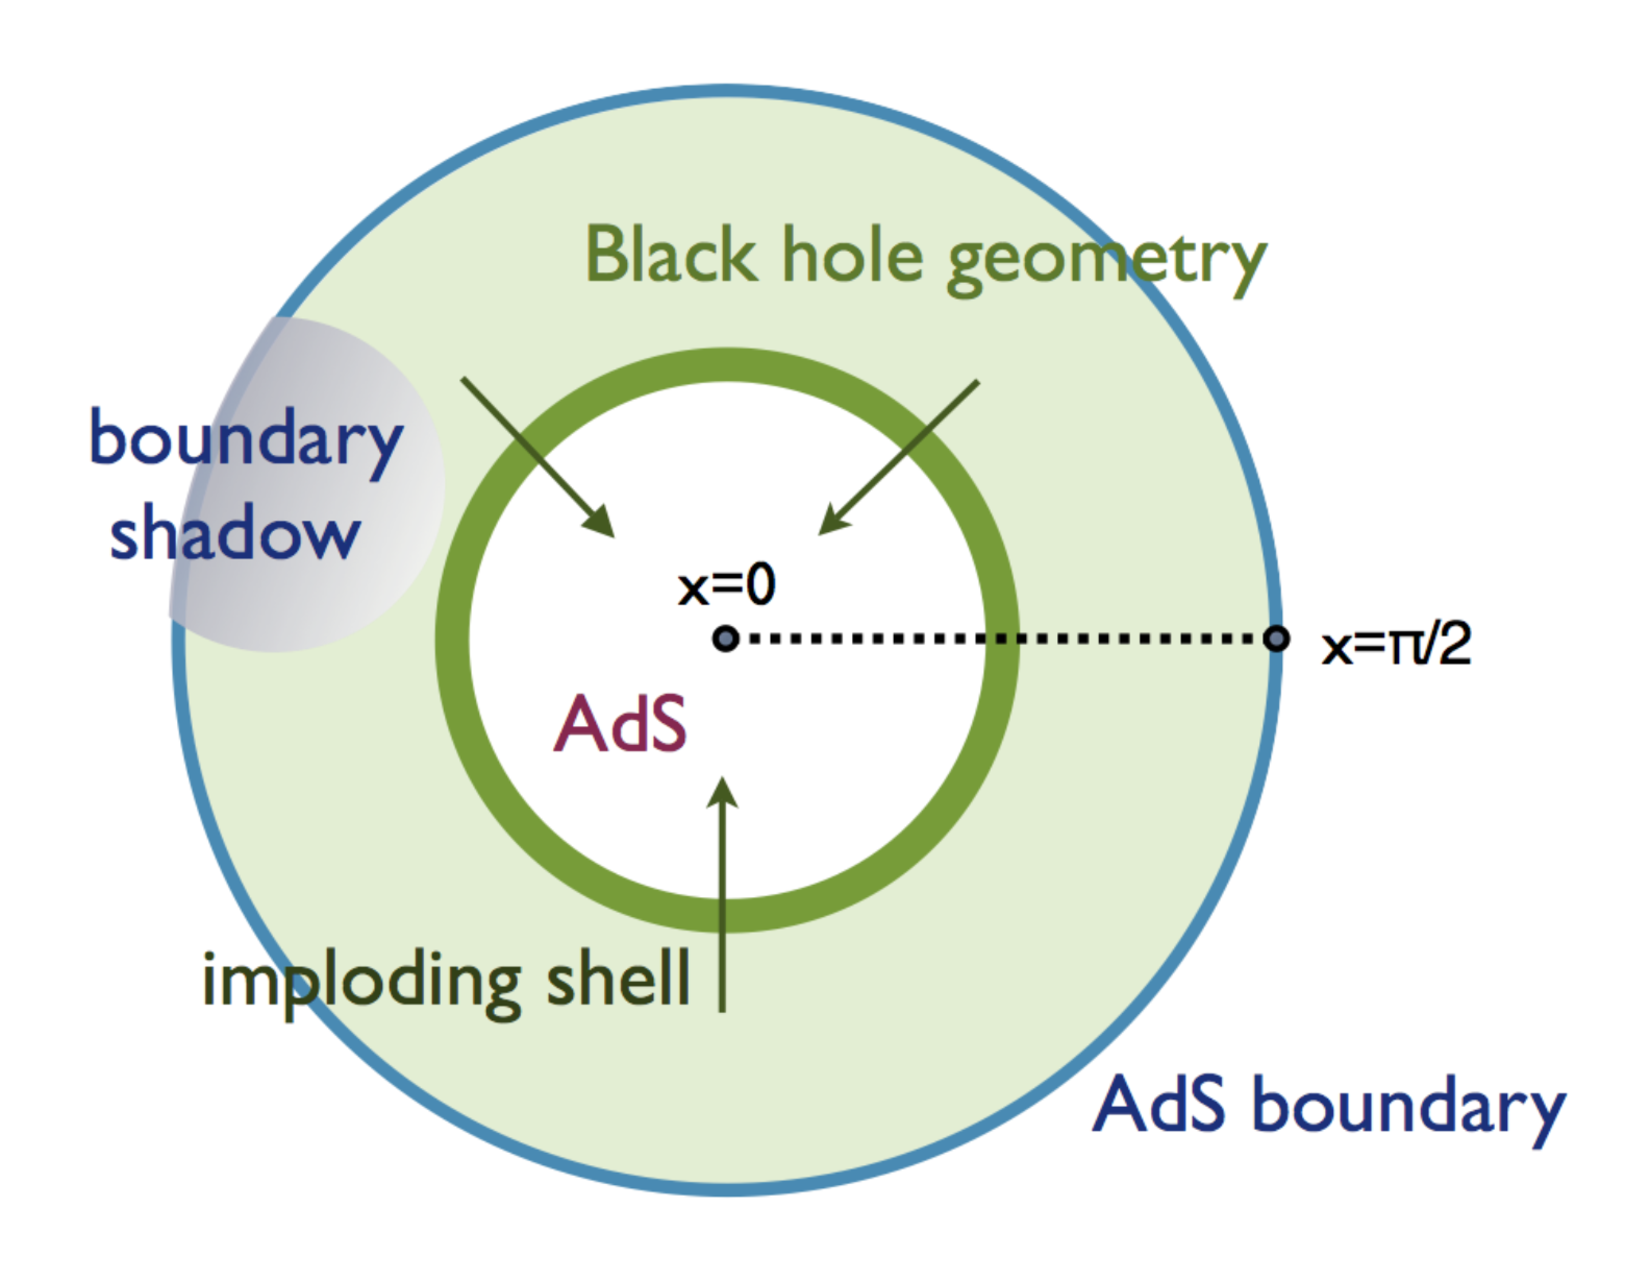
\includegraphics[width=0.5\textwidth]{/Users/bradc/Research/Thesis/PhD/Intro/figs/EE.pdf}	
	\caption[Gravitational picture of a holographic quantum quench in a CFT]{An infalling spherical shell can scatter of itself and begin expanding, eventually reaching the conformal boundary where it is reflected back and begins imploding again {\rm \cite{1412.6002}}.}
	\label{fig: EE}
\end{figure}

Besides studying thermalizing systems, scalar field collapse can also be used to examine revivals in quantum systems away from equilibrium, and thus help explain the results from cold atom experiments, {\it e.g.} \cite{Dziarmaga2010, 2011arXiv1106.3567L}. Holographic quenches and revivals can also be used to confirm non-holographic results, such as the study of free, spinless Majorana fermions bound as pairs in meson excitations \cite{1706.02438}. Finally, we may wish to investigate the evolution of one thermal state into another, such as evolving from a non-hairy black hole in AdS to a hairy black hole -- a process equivalent to the spontaneous breaking of a discrete symmetry \cite{1704.05454}.

Using various nonlocal holographic probes, such as entanglement entropy, the time evolution of the quantum properties of the boundary theory can be determined \cite{1410.6201}. For example, \cite{1412.6002} uses the implosion of a spherical shell of matter to study quenches in confined gauge theories. Figure~\ref{fig: EE} is a schematic representation of the holographic theory. The radial position of the shell in the bulk acts as a scale to measure the typical separation of entangled excitations. As the shell falls towards $x = 0$, one of two things can happen: if the shell has a high enough mass density, a black hole forms which signals the thermalization of the gauge theory; if the shell does not collapse, it can scatter off itself and begin expanding. Once the shell reaches the AdS boundary, the matter is reflected (under appropriate boundary conditions) and begins the infall again. This cycle of bounces is the holographic dual of so-called \emph{revivals} in the quantum theory.

Note the boundary shadow region included in figure~\ref{fig: EE}. This area represents where holographic computations are done for a given interval on the boundary. Recall from \S~\!\ref{ssub: EE} that the geometric dual to entanglement entropy in some interval is a quarter of the minimal surface in the bulk anchored to the boundary interval. As the mass shell evolves and backreacts with the geometry, this minimal surface also evolves. Although the exact details depend on the number of dimensions, numerical results for AdS$_3$ and AdS$_4$ both show that the entanglement entropy reaches a maximum when the radial position of the spherical shell is equal to the maximum distance of incursion into the bulk by the extremal surface.

%%%%%%%%%%%%%%%%%%%%%%%%%%%%%%%%%%%%%%%%%%%%%%%%%%%%%%%

\subsection{Scalar Fields in AdS$_{d+1}$}

Let us now establish the particulars of the gravitational dual to a coherent state in the boundary CFT. Following \cite{1508.02709}, we begin by writing the metric of AdS$_{d+1}$ in Schwarzschild-like coordinates 
\begin{align}
ds^2 = \frac{\ell^2}{\cos^2 \left(x / \ell \right)} \left( A e^{-2\delta} dt^2 + A^{-1}dx^2 \sin^2 \left(x / \ell \right) d\Omega^{d-1} \right) \, ,
\end{align}
where $x \in [0, \pi/2)$ and $x = \pi / 2$ corresponds to the conformal boundary. The metric functions $A(t,x)$ and $\delta(t,x)$ are functions of only two variables due to the spherical symmetry. We will hereafter work in units of the AdS length scale, setting $\ell = 1$. The Einstein and Klein-Gordon equations for the minimally-coupled scalar field $\phi(t,x)$ are
\begin{align}
G_{ab} + \Lambda g_{ab} = 8\pi \left( \nabla_a \phi \nabla_b \phi - \frac{1}{2} g_{ab} \big( \left( \nabla \phi \right)^2 + \mu^2 \phi^2 \big) \right) \quad \text{and} \quad \frac{1}{\sqrt{-g}} \p_a \sqrt{-g} \, g^{ab} \p_b \phi - \mu^2 \phi = 0 \, .
\end{align}
The canonical equations of motion are \cite{1210.1566}
\begin{align}
\label{canon eqns}
\p_t \phi = A e^{-\delta} \Pi \, , \quad \p_t \Phi = \p_x \left( A e^{-\delta} \Pi \right) \, , \quad \text{and} \quad \p_t \Pi = \frac{\p_x \left( \Phi A e^{-\delta} \tan^{d-1} (x) \right)}{\tan^{d-1}(x)} - \frac{\mu^2 e^{-\delta} \phi}{\cos^2 (x)} \, ,
\end{align}
where the momentum is $\Pi(t,x) = A^{-1} e^{\delta} \p_t \phi$ and $\Phi(t,x) \equiv \p_x \phi$. The metric functions obey
\begin{align}
\label{metric funcs}
\begin{gathered}
\p_x \delta = - (\Pi^2 + \Phi^2 ) \sin (x) \cos(x) \, , \quad A = 1 - \frac{2M \sin^2 (x) }{(d-1) \tan^{d-1}(x)} \\
\p_x M = \tan^{d-1}(x) \left[ \frac{A (\Pi^2 + \Phi^2)}{2} + \frac{\mu^2 \phi^2}{2 \cos^2 (x)} \right] \, ,
\end{gathered}
\end{align}
with the mass function $M(t,x)$ subject to the conservation equation $\p_t M( t, x = \pi/2) = 0$. The value of $\delta(t,x)$ is chosen to correspond to the interior gauge, {\it i.e.} $\delta(t,x=0) = 0$. 

\subsection{Stable Configurations}

Consider perturbative solutions to $\{$\eqref{canon eqns}, \eqref{metric funcs}$\}$ arising from expanding the scalar field and metric functions via
\begin{align}
\phi(t,x) = \sum_{j=0}^{\infty} \epsilon^{2j + 1} \phi_{2j + 1} (t,x) \, , \quad A(t,x) = 1 - \sum_{j=1}^\infty \epsilon^{2j} A_{2j} (t,x) \, , \quad \delta(t,x) = \sum_{j=1}^\infty \epsilon^{2j} \delta_{2j} (t,x) \, ,
\end{align}
where $\epsilon$ is a (small) constant. At linear order, the gravitational system obeys
\begin{align}
\label{collapse eigen eqn}
\p_t^2 \phi_1 = \left( \frac{ (d-1)}{\sin (x) \cos (x)} \p_x + \p^2_x - \frac{\mu^2}{\cos^2 (x)} \right) \phi_1 \equiv - L \phi_1 \, ,
\end{align}
whose normalized eigenfunctions are the Jacobi polynomials
\begin{align}
\label{scalar eigens}
e_j (x) = k_j \cos^{\lambda_\pm}(x) P_j^{(\frac{d}{2} - 1, \lambda_\pm - \frac{d}{2})} \left( \cos \left( 2x \right)\right) \, .
\end{align}
The eigenvalues have the simple form $\omega_j = \lambda_\pm + 2j$, with $\lambda_\pm = (d \pm \sqrt{d^2 + 4\mu^2})/2$ ({\it cf.} mass dimension and the Breitenlohner-Freedman bound for scalar fields in \S~\!\ref{ssec: scalar fields}). 

Solutions to the linearized equations of motion are stable to linear order on the timescale $t \sim \epsilon^{-2}$ \cite{1506.07907}. However, beyond linear order there are instabilities at $\mc O(\epsilon^3)$ due to secular terms, which are terms that grow larger with time. These terms cannot be removed by frequency shifts and arise from resonances in the spectrum of the scalar fields  \cite{1407.6273}. Various resummation \cite{hep-th/9506161} and multi-scale techniques \cite{1403.6471} have been developed to help control growth of terms; however, there is some debate about the numerical confirmation of these solutions in the full theory.

\subsubsection{Oscillons, Oscillatons, and Geons}
\label{sub: geons}

When $\mu = 0$ in \eqref{collapse eigen eqn}, we recover the \emph{oscillon} solution \cite{1701.09100}. Oscillons are long-lived and nearly time-periodic solutions. Further work has demonstrated that single oscillon solutions emit energy very slowly, leading to corresponding decreases in the amplitude and period of the solutions \cite{hep-ph/9503217}. A oscillon solution is stable over very long time scales; however, if a solution is constructed out of a linear combination of oscillons, the system exhibits possible third-order instabilities on the same timescale as the linearized solutions. These instabilities, however, can be absorbed by a frequency shift. Therefore, oscillons are non-linearly stable. A similar class of solutions, called \emph{oscillatons}, are oscillating, localized solutions for massive scalar fields, but are generic to backgrounds that are asymptotically flat. Oscillatons also remain stable over long time scales \cite{gr-qc/0310006}.

More general oscillating solutions exist as solutions to Einstein-Maxwell equations in a vacuum. These solutions, known as \emph{geons}, are high-frequency gravitational waves that are confined to a background geometry created by the waves themselves \cite{Wheeler:1955zz}. Geon solutions for AdS have been established by \cite{1109.1825} and are at least perturbatively stable at first order. Like the oscillons, geons exhibit instabilities at third order. By invoking various resummation techniques to account for the growth of secular terms at third order, there has been some success with constructing nonlinearly stable solutions for certain initial data \cite{1408.5906, 1701.07804}. Non-linearly stable numerical solutions in a number of different dimensions can also be derived from perturbing away from geon solutions \cite{1503.07746}.

\subsubsection{Boson Stars}

Boson stars are a class of localized, stationary, nonlinearly stable solutions involving complex scalar fields. Since the \ads action is invariant under the global phase transformation $\phi \to \exp(-i \theta) \phi$, boson stars carry a conserved charge, $Q$. They have since been numerically constructed and shown to be stable solutions to the full, nonlinear theory \cite{1304.4166}. They can be constructed from a range of initial conditions \cite{1209.2378, 1301.2452} and do not suffer from Gregory-Laflamme instabilities (see \S~\ref{sub: extra dims on stability} for details on how instabilities in the non-AdS dimensions may affect our understanding of holographic thermalization) \cite{1509.00774}. 

\subsubsection{Single-mode and Nearly Single-Mode Data}

Stable, time-periodic solutions for scalar fields that were not based on linear solutions came from postulating an expansion for the scalar field that is dominated by a single mode in the limit of vanishing amplitude. This type of solution is referred to as single-mode solutions. By solving the system of linear equations -- using, for example, Newton-Raphson or Broyden optimizing algorithms -- we can determine the coefficients of the first $N$ terms in the expansion. This serves as the starting point for the pseudo-spectral or finite difference numerical evolution. Using this method, stable, single-mode solutions in AdS$_5$ were constructed and evolved in time. The solutions were found to be periodic and numerical evidence suggests they remained nonlinearly stable \cite{1303.3186}.

Nearly single-mode solutions are similar to single-mode solutions in that they are dominated by a small number of modes in the limit of vanishing amplitude. Using nearly-single mode initial data for complex scalar fields, \cite{1304.4166} then numerically evolved the full, nonlinear system and found that these solutions were fully stable for sufficiently small perturbations.

\subsubsection{Gaussian Initial Data}

It was asserted by \cite{1106.2339} that scalar fields with small amplitudes were generically stable in AdS$_5$. This conclusion was proven to be false by \cite{1108.4539}, who showed that all fields with Gaussian initial momentum profiles collapsed for any AdS$_{d+1}$ with $d \geq 3$. What was initially missed was that low-amplitude fields could be focused, scatter out to the boundary, then be reflected back multiple times before finally collapsing. It was only by continuing simulation times to orders of magnitude more than the light crossing time that collapse was eventually witnessed. We will see in \S~\ref{ssub: islands} below that the behaviour of Gaussian initial data is, in fact, more nuanced than generic stability or instability.

By generalizing the geometry of the bulk space \emph{asymptotically} AdS spaces, some scalar field configurations with Gaussian initial data were found to be nonlinearly stable \cite{1208.5772}. This was because the resonances that plagued solutions in strict AdS had been sufficiently misaligned to resist collapse. 

%%%%%%%%%%%%%%%%%%%%%%%%%%%%%%%%%%%%%%%%%%%%%%%%%%%%%%%
 
\subsection{Unstable Configurations}
\label{sub: numerical}

As we have seen, although linearly stable, long-lived solutions exist for asymptotically AdS gravitational theories, all suffer from third-order instabilities. While these instabilities can be controlled in some scenarios, it is not clear that analytical solutions can be derived in general. This type of behaviour is called a \emph{weakly turbulent} instability because of its appearance at higher orders. What results is a transfer of energy from low eigenmodes to high ones, a process referred to as an energy cascade. With more energy transferred to higher frequencies, the energy density becomes sufficiently great to trigger the formation of an apparent horizon and, eventually, a black hole.

The earliest examination of black hole formation from scalar field collapse using numerical methods was done on a flat background. For generic initial data parameterized by $p$, the following critical phenomena were observed by \cite{Choptuik:1992jv} for spherically-symmetric solutions:
\begin{itemize}
\item If collapse is guaranteed for values $p > p^*$, then as $p \to p^*$, black holes can be created with masses $M \propto |p - p^*|^\gamma$. The critical exponent $\gamma$ is independent of initial conditions and depends only on the type matter. For spherically symmetric, massless scalar field, $\gamma \approx 0.37$.
\item Just before the formation of the event horizon, the spacetime approaches a scale-invariant solution -- the critical solution -- that is also independent of the initial conditions.
\end{itemize}

These characteristics are collectively known as Choptuik scaling, and have also been observed in critical solutions in AdS spacetimes, independent of initial conditions.

\subsubsection{Complex Scalars}

Complex scalar fields in AdS$_{d+1}$ with $d \in [3,\ldots,6]$ and generic Gaussian initial data -- \emph{not} boson star solutions -- were examined by \cite{1210.0890}. When the effect of the conserved charge was included, it was shown that the rate of collapse was greater for charged scalars than for uncharged scalars. The generic instability of the spaces was also confirmed, since all solutions lead to collapse in the full, nonlinear theory. To probe the nature of the instability, scalar fields in AdS were considered, but with a reflective boundary at a finite distance. The result was the observation of turbulent cascade of energy to shorter wavelengths and collapse to a black hole. However, when $Q = 0$, a threshold amplitude for black hole formation was found and scalar fields did not collapse. This contradicts the result of \cite{1208.2934}, who examined scalar field in flat space but with a reflective boundary. While turbulent cascades were also noted in that case, there was no threshold amplitude.

\subsubsection{Gaussian Initial Data Revisited}

The first examination of the time evolution of a massless scalar solution in AdS$_4$ returned a surprising result: for any scalar field with Gaussian initial momentum profile, the formation of a black hole was inevitable, even for amplitudes of order $\epsilon$ \cite{1104.3702}. This was a deviation from the flat background result, which required a minimum energy density in order for a black hole to form. In figure~\ref{fig: x vs eps}, the horizon size $x_H$ is plotted as a function of initial scalar field amplitude, $\epsilon$. Near criticality, when the amplitude $\epsilon$ is close to the amplitude $\epsilon_0$ that produces a black hole with radius $r_+ \to 0$, scale invariance of the solution was observed in agreement with the asymptotically flat results. Universal scaling of the horizon size (and therefore mass) was also confirmed. 

To test the robustness of the solutions to changes in initial conditions, a phase diagram of initial profiles for real, massless scalar fields in AdS$_5$ was constructed by \cite{1106.2339} and improved upon by \cite{1110.5823}. The initial profile of the scalar field was taken to be $\phi(t=0, x) = \epsilon \exp \big( -(x^2 - x_0^2) / \sigma^2 \big)$, where $x_0$ is the centre of the profile. By varying the value of $\epsilon$ or $\sigma$ while holding the other constant, the strength of the dependence of horizon formation time and size on these two parameters was determined. Qualitatively, it was found that the formation time depended more strongly on the amplitude than the width. 

While some of the disagreement regarding the stability of certain initial data was due to modelling errors or other factors, there was some indication that there might exist a finite number of configurations within an unstable profile that were stable over long periods. 

\subsubsection{Islands of Stability}
\label{ssub: islands}
 
In \cite{1508.02709}, a large swath of the phase space of Gaussian data of the type
\begin{align}
\label{scalar ics}
\phi(t=0,x) = 0 \quad \text{and} \quad \Pi (t=0,x) = \epsilon \exp \left( - \frac{\tan^2 (x)}{\sigma^2} \right)
\end{align}
was explored down to very low amplitudes in AdS$_4$ and AdS$_5$. Surveying such a wide range of masses and widths allowed for the confirmation of the periodic, discontinuous horizon behaviour observed for massless scalars in \cite{1104.3702}, as well as observing similar behaviour for light masses ($\mu < 1$) with both narrow widths ($\sigma \approx 0.3$) and wide widths ($\sigma \approx 4$). New, quasi-stable behaviour was found for heavy masses ($\mu = 20$) at intermediate widths, which was characterized by discontinuous behaviour in horizon formation time where fields with initial amplitudes in a small range experienced jumps in formation time of orders of magnitude. Finally, for very heavy scalars ($\mu = 100$), a threshold amplitude was found below which no black hole solution was seen. See figure~\ref{fig: massive x vs eps} for one such example.

\begin{figure}[h]
	\centering
	\begin{subfigure}[t]{0.45\textwidth}
		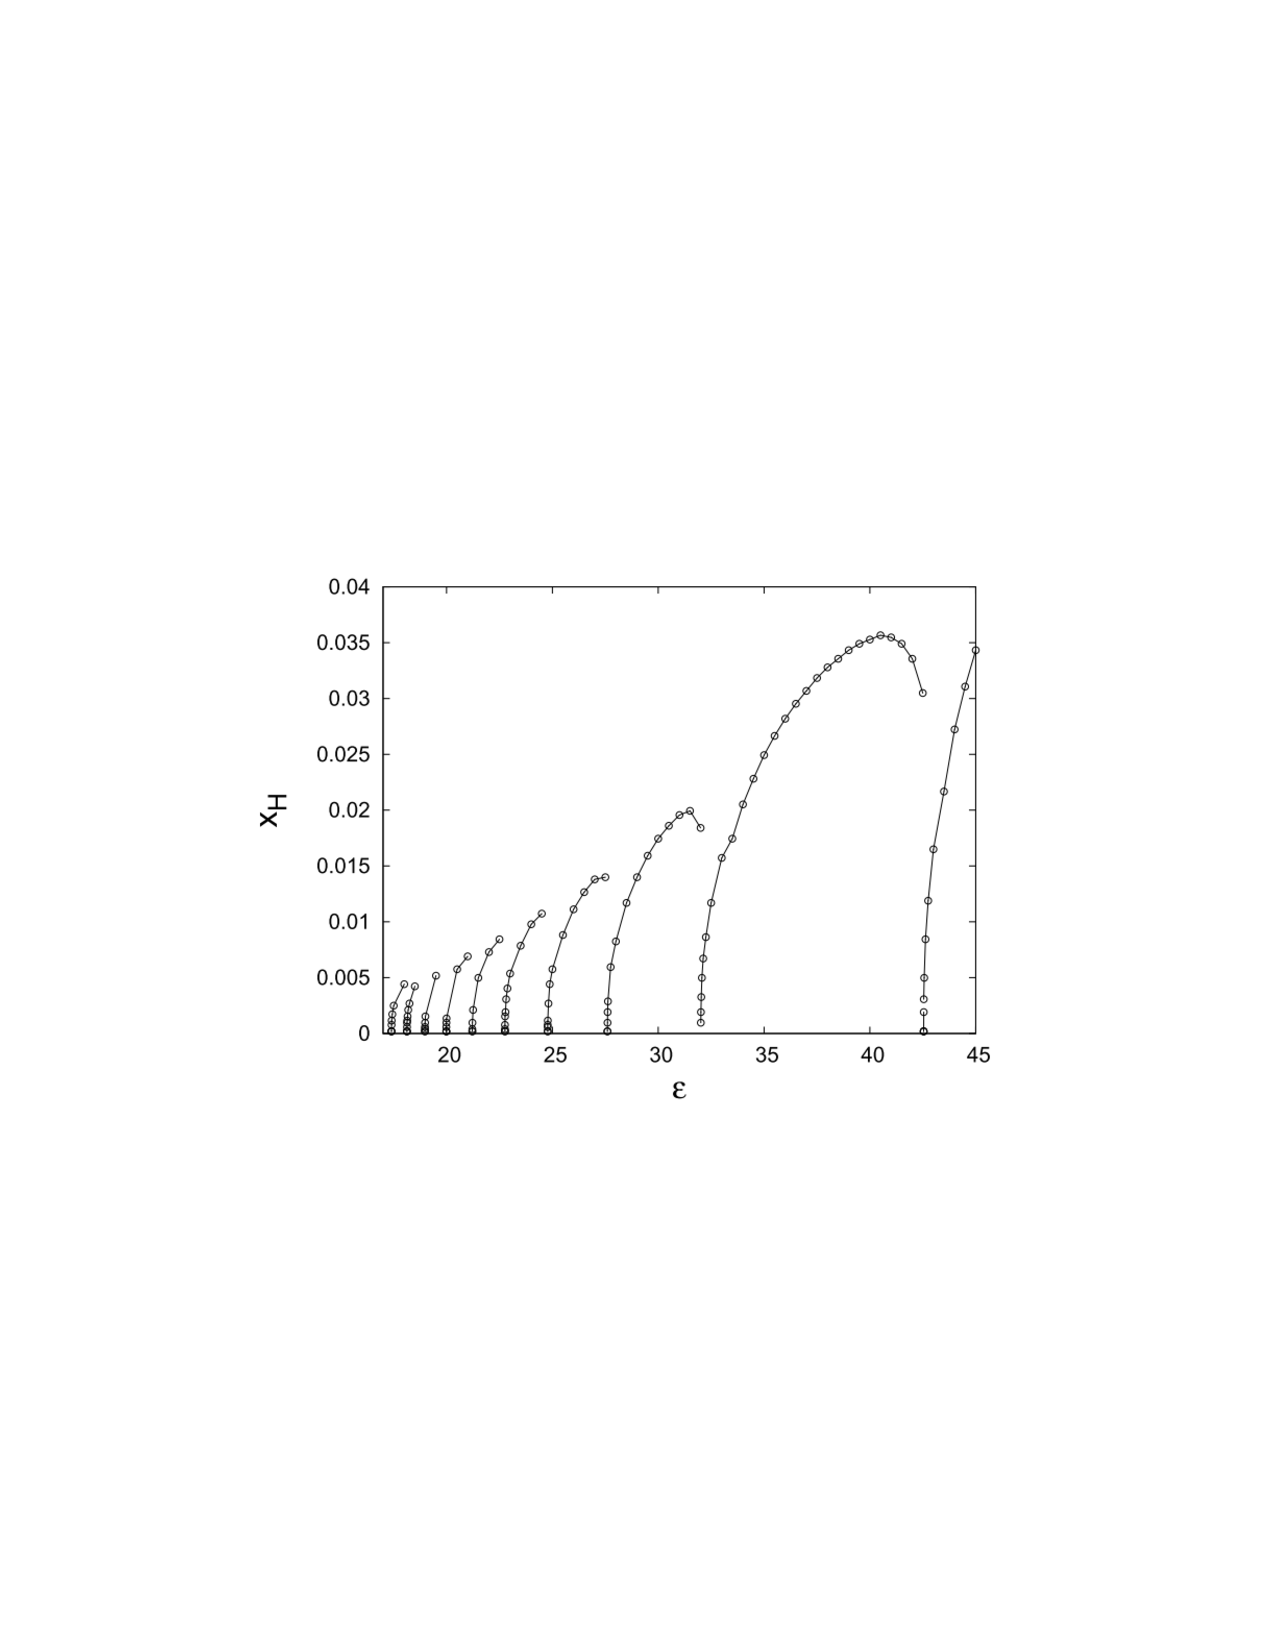
\includegraphics[width=\textwidth]{/Users/bradc/Research/Thesis/PhD/Intro/figs/bizon_horizonvsepsilon}	
		\label{fig: x vs eps}
	\end{subfigure} 
	\;
	\begin{subfigure}[t]{0.45\textwidth}
		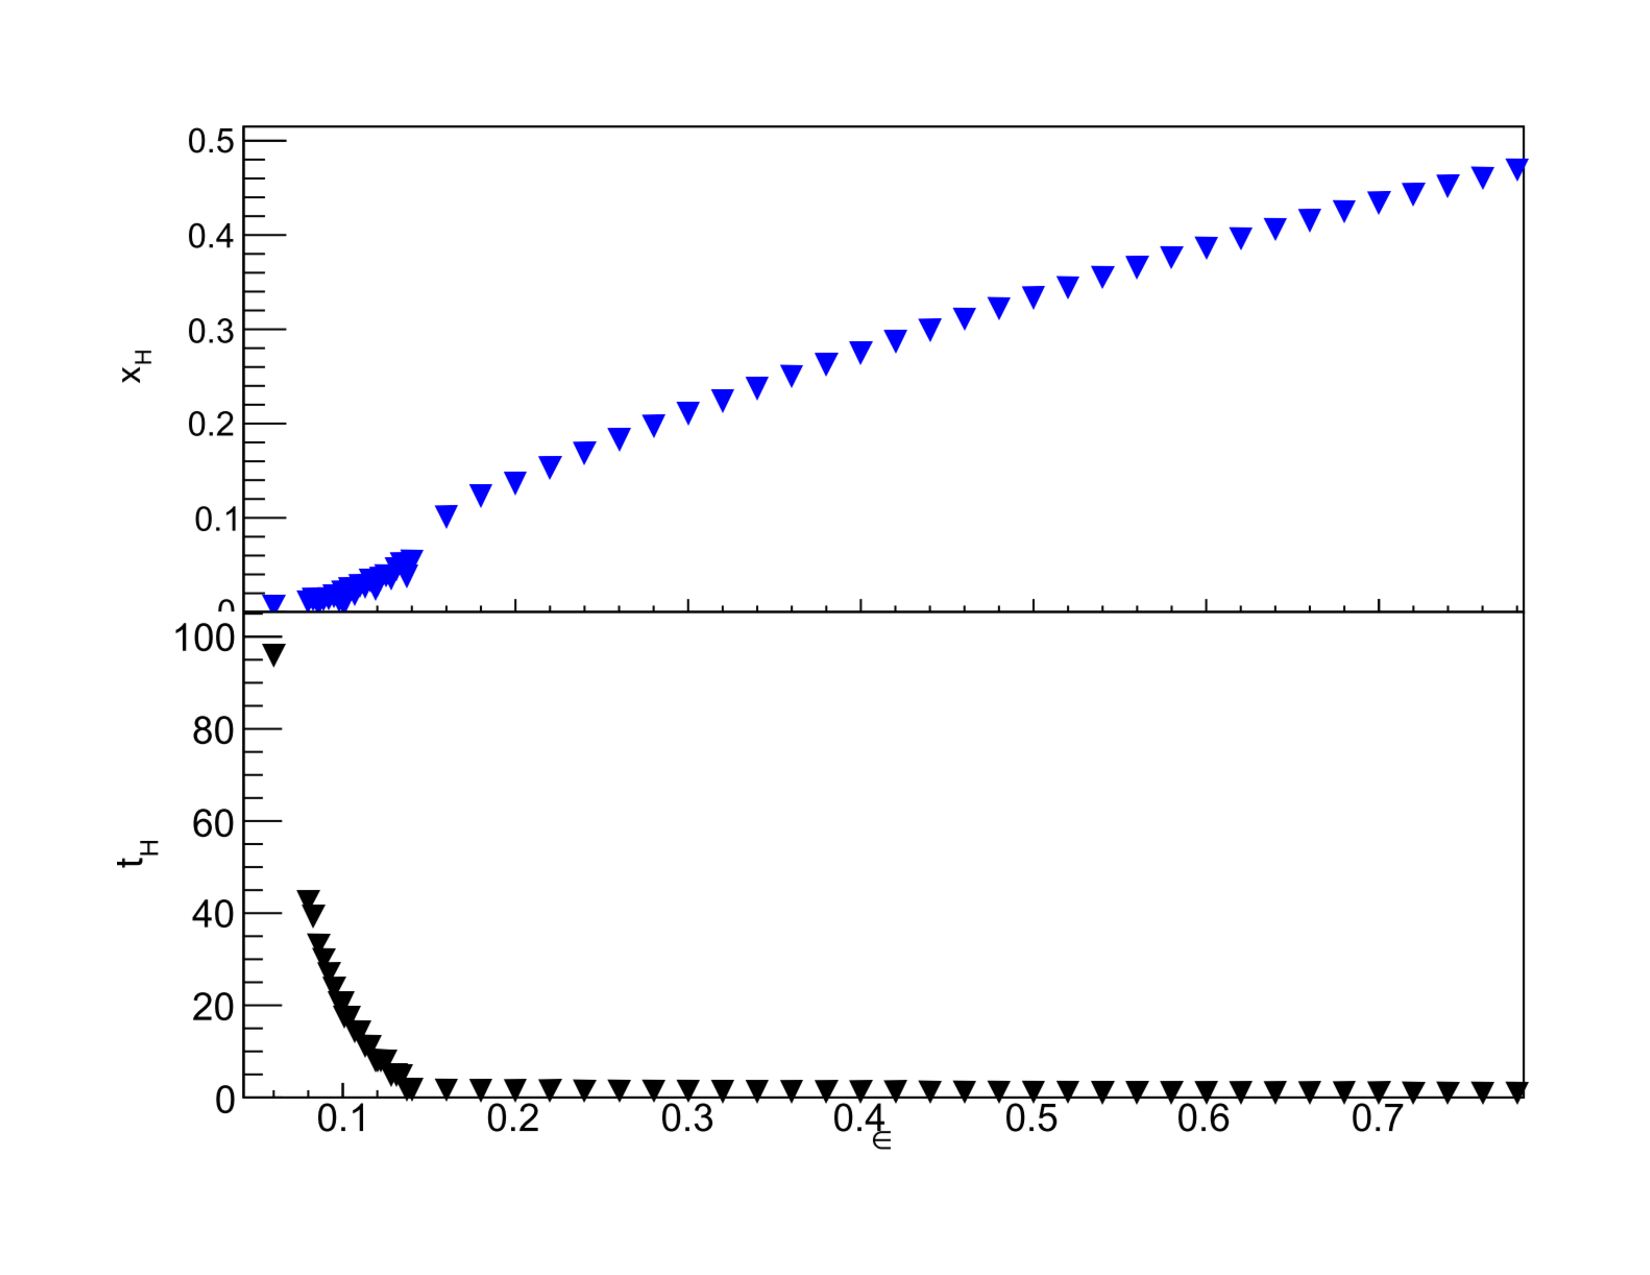
\includegraphics[width=\textwidth]{/Users/bradc/Research/Thesis/PhD/Intro/figs/massive_x_vs_eps.pdf}
		\label{fig: massive x vs eps}
	\end{subfigure}
	\caption[Horizon size and horizon formation time for massless and massive scalars]{Left: The behaviour of horizon size with amplitude for massless scalars observed by {\rm\cite{1104.3702}}. The critical value $\epsilon_0$ is the first instance when $x_H = 0$. There are further critical values found by continuing to decrease the amplitude. The difference in horizon formation times between successive critical values is $t(\epsilon_{i+1}) - t(\epsilon_i) \approx \pi$, the light-crossing time. Right: Horizon size and horizon formation time as a function of amplitude in AdS$_5$ for a massive scalar field and $\sigma = 2$ in {\rm\eqref{scalar ics}}. Instead of the periodic, discontinuous behaviour, there is some minimal value $\epsilon_{min}$ below which black holes to not form {\rm\cite{1508.02709}}.}
\end{figure}

A picture of phase space for initial profiles of scalar fields has emerged: Gaussian data describing either narrow or wide pulses will always lead to collapse on the timescales corresponding to turbulent cascades of energy to shorter wavelengths; however, there is a set of intermediate widths that exhibit stable behaviour below some critical amplitude, at least to time scales on the order of $t \sim \epsilon^{-2}$. These solutions are referred to as ``islands of stability.'' Interpreting the balance between energy flowing between short and long wavelengths that allows for such solutions to be stable remains a subject of ongoing research \cite{1507.08261, TTF, 1706.07413, 1912.07143}.

\subsubsection{Two-Mode Initial Data}

Two-mode initial data uses initial profiles of the form $\phi(t=0,x) = \epsilon ( e_0 (x) + \kappa e_1 (x) )/3$, where $\kappa$ is a free constant and $e_0(x), \: e_1(x)$ are the first two eigenmodes of \eqref{scalar eigens}. While initial results by \cite{1403.6471} indicated that such data was stable for $\kappa \sim 1$, it was pointed out by \cite{1410.2631} that  collapse did indeed occur. It was postulated that the observed stability was a result of too coarse a mesh and/or ineffective adaptive mesh refinement, resulting in the apparent horizon falling between grid points of the simulation. The instability of two-mode solutions was subsequently confirmed in \cite{1508.02709}.

%%%%%%%%%%%%%%%%%%%%%%%%%%%%%%%%%%%%%%%%%%%%%%%%%%%%%%%

\subsection{Beyond Spherical Symmetry}
\label{sub: beyond spherical}

As we have seen, the AdS/CFT correspondence imposes conditions on the asymptotic properties of the bulk space. However, this leaves open the possibilities for interior geometries outside of the spherically-symmetric ones we have considered so far. By studying background with different symmetry properties, we will be able to differential between what behaviour is intrinsic to the gravitational theory, and what behaviour depends on the matter profile.

Threshold behaviour for axisymmetric scalar fields in flat geometries has confirmed the existence of critical phenomena of the type outlined in \S~\!\ref{sub: numerical}. In addition to confirming scale invariance for critical solutions, a critical exponent of $\gamma \approx 0.11$ was found \cite{gr-qc/0405101}. Further work examining axisymmetric vacuum solutions found critical behaviour of the same form, but with critical exponent $\gamma \approx 0.37$ \cite{Abrahams:1993wa}.

In a more systematic study carried out in AdS$_5$, the degree of deformation away from spherical symmetry was included as an independent variable \cite{1706.04199}. While holding mass constant, it was shown that scalar fields collapsed to form black holes at earlier times and with fewer bounces as the deviation from spherical symmetry increased. By then considering data that required a fixed number of bounces to collapse, the effect of increased asymmetry isolated. The conclusion was that less mass was required to trigger a collapse after a fixed number of bounces as the degree of asymmetry was increased.

More recently, a systematic approach to treating higher-order gravitational perturbations beyond spherical symmetry was developed by \cite{1701.07804}. Using axisymmetric solutions as an example of the method, time-periodic vacuum solutions -- {\it i.e.}, geon solutions -- were constructed. In such a system, the eigenvalues of the linear perturbations are degenerate as they depend not only on mode number, but also on the number of radial nodes, and the choice of either polar or axial modes. It was shown that the stable, time-periodic solutions are described by one-parameter families of solutions for each frequency, with the number of families equal to the multiplicity of the linear eigenfrequency.

Finally, by breaking both spherical \emph{and} axial symmetry, the nonlinear instabilities due to secular terms become much stronger \cite{1705.03065}. In contrast to the spherically symmetric case, even single-mode data develop irremovable resonances at third order that lead to collapse.

\subsubsection{Boson Stars Without Spherical Symmetry}

Numerical boson star solutions with axisymmetry are able to incorporate the effects of angular momentum on the collapse of the scalar field. For an axisymmetric boson star data with momentum $J \propto \epsilon^2$, \cite{1706.06101} has shown that the timescale for collapse remains $t \sim \epsilon^{-2}$. Furthermore, as with spherically-symmetric oscillons, there are numerical solutions that are extensions of normal modes that remain stable over longer timescales. 

The collapse of unstable boson star-like fields with angular momentum is sensitive to the type of perturbation applied, and may react by either collapsing to a Myers-Perry black hole, or by continuing to oscillate. For collapses in the full, nonlinear theory, critical phenomena such as self-similarity and mass scaling continue to hold \cite{gr-qc/0410040}. As the angular quantum number of the boson star solutions is increased, the resulting black hole is more and more distorted; in particular, the black hole develops multiple ``lobes'' about its centre that do not settle into more symmetric configurations due to the boundary properties of AdS \cite{1202.5809}. When considering oscillating solutions, it has been suggested that boson stars with angular momentum may continue to oscillate indefinitely, rather than tend towards radially-static solutions like the $J = 0$ case.

\subsubsection{Extensions of Einstein's Gravity}

In addition to considering various symmetry properties of solutions, the collapse of scalar fields in AdS has been extended to modified gravitational theories. One such extension was a generalization of the Einstein-Hilbert action to include higher-order curvature terms, {\it i.e.} Einstein-Gauss-Bonnet gravity. In such theories, \cite{1410.1869} has demonstrated the existence radius gaps in the near-critical scaling, thereby excluding black holes of arbitrarily small masses. Furthermore, for states below the mass threshold, gravitational focusing and growth of background curvature at late times suggest that either \emph{a}) naked singularities may develop, or \emph{b}) the curvature becomes sufficiently large excite string degrees of freedom, resulting in the end state being a gas of strings \cite{1608.05402}.

%%%%%%%%%%%%%%%%%%%%%%%%%%%%%%%%%%%%%%%%%%%%%%%%%%%%%%%

\subsection{The Effects of Extra Dimensions on Stability}
\label{sub: extra dims on stability}

While our focus has mainly been on dynamics in the AdS dimensions, we must not forget that the full spacetime is actually ten-dimensional. Let us step back from the example of \ads for a moment to examine what effects the dynamics in AdS might have on the other dimensions.

Consider the 10D background to be the product of two generic 5D manifolds $\mc M_5 \times \mc V_5$. The vacuum solution supports a 5-form flux and has the geometry $\mc M_5 =$ AdS$_5$; the dual strongly-coupled gauge theory lives on the conformal boundary $\p \mc M_5$. The details of the gauge theory depend on the choice of geometry for $\mc V_5$ since the central charge of the CFT is inversely related to the volume of $\mc V_5$. When $\mc V_5 =$ S$^5$, the gauge theory is an $\mc N = 4$, super-Yang-Mills theory. In the full 10D theory, when black holes form in the AdS$_5$ space, they are smeared across the $\mc V_5$. 

In the small horizon limit, $r_+ \to 0$, the black hole will suffer a Gregory-Laflamme instability that causes the smeared solution to collapse to a point on S$^5$ \cite{hep-th/9301052}. This instability has been verified for \ads and generalized to arbitrary 5D manifolds \cite{1509.07780}. The threshold size for the instability to take effect is given by the size of the leading-order fluctuation; for \ads in particular, this is $r_+ / \ell \simeq 0.4259$ \cite{1502.01574}. The implication of the Gregory-Laflamme instability is that, for black holes of size (or, equivalently, mass) less than or equal to the instability size, collapse in the extra dimensions would precede collapse in the Anti-de Sitter dimensions, leading to a naked singularity. Such a violation of cosmic censorship would call the entire holographic description of quantum quenches into question. However, this effect as yet to be observed in numerical studies and might be avoided if the scalar field in AdS space develops a horizon before the Gregory-Laflamme collapse produces a singularity. Such a comparison has yet to be directly addressed in the literature, and may be the subject of future work by this author.

A similar instability scale has been established for boson star configurations using the SUGRA effective action in 10D coupled to a complex scalar field. Once again, the threshold size is determined by examining the lowest-order contribution to the spectrum of linearized fluctuations. In contrast to the Gregory-Laflamme-type instabilities, localization on compact dimensions is observed \emph{above} a threshold mass \cite{1509.00774}.

%%%%%%%%%%%%%%%%%%%%%%%%%%%%%%%%%%%%%%%%%%%%%%%%%%%%%%%
%%%%%%%%%%%%%%%%%%%%%%%%%%%%%%%%%%%%%%%%%%%%%%%%%%%%%%%

\section{Summary}
\label{sec: summary}

In this review, we have seen how the AdS/CFT correspondence establishes a duality between strongly-coupled gauge theories and weakly-coupled gravitational theories in one extra dimension. Using this correspondence, various dynamical processes in strongly-coupled gauge theories can be explored via the collapse of scalar fields in Anti-de Sitter space. In particular, we have focused on the duality between the formation of black holes from scalar fields in \ads and the thermalization of an $\mc N = 4$, super-Yang-Mills theory in four dimensions. We have seen that the end state of the theory depends on the initial profile of the scalar field, and that a large variety of both stable and unstable phenomena are possible. Finally, we have seen that lingering questions about the role of bulk symmetries and the nature of instabilities in the full, 10D theory mean that there are more exciting avenues of research yet to be explored.

%%%%%%%%%%%%%%%%%%%%%%%%%%%%%%%%%%%%%%%%%%%%%%%%%%%%%%%
%%%%%%%%%%%%%%%%%%%%%%%%%%%%%%%%%%%%%%%%%%%%%%%%%%%%%%%



\end{document}

%%%%%%%%%%%%%%%%%%%%%%%%%%%%%%%%%%%%%%%%%%%%%%%%%%%%%%
%%%%%%%%%%%%%%%%%%%%%%%%%%%%%%%%%%%%%%%%%%%%%%%%%%%%%%
